\section{Learning set creation}
    \subsection{Table creation}
        We now have a denoised dataset 19 column table. Our mission now to unroll it in to a long table with 2 columns, the first one is the name of the electrode and the others is the value. The melt function is used to do this. We change the variable to match the class from 0 to 3 as below:
        
        \begin{itemize}
        \item Class 0: including FP1-AVE, FP2-AVE, F3-AVE, F4-AVE, F7-AVE, F8-AVE, Fz-AVE
        \item Class 1: including C3-AVE, C4-AVE, Cz-AVE
        \item Class 2: including T3-AVE, T4-AVE, T5-AVE, T6-AVE
        \item Class 3: including P3-AVE, P4-AVE, Pz-AVE, O1-AVE,  O2-AVE
    \end{itemize}

        \begin{figure}[h]
        \centering
        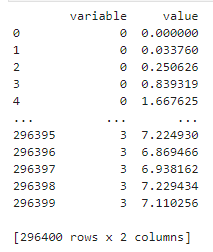
\includegraphics[width = 0.3\textwidth]{images/unroll.png}
        \caption{Unrolled dataset}
        \label{fig:unroll}
        \end{figure}
        
        Figure~\ref{fig:unroll} illustrate a part of the signal after unroll the signal. The first column will be variable, which is indicates the class of the data step. The second column indicates the value of the data steps itself.
      
      In this specific article, This dataset will be divide into multiple time window frame W with multiple data steps in order to create multiple data points so we can apply machine learning method. We will test in 2 type of time windows W to see if there is any difference.
      
      \begin{itemize}
          \item Time window W1: 200 steps each
          \item Time window W2: 400 steps each
      \end{itemize}
      
      \subsection{Shuffling}
        To make the data reduce variance and making sure the model general and less over fit, We will need to shuffle the data before do any further. Fortunately, python has built-in a random library and it make us more easy.
        
        \begin{lstlisting}
        import random
        random.shuffle(training_data)
        \end{lstlisting}
        
        With time windows W1, we have 1482 data points and with time windows W2, we have 741 data points. I will separate around 20\% of the dataset we have here to create a testing set, and the other 80\% will be training set. Thus, W1 have 1282 points in training set and 200 points in testing set, and the others W2 will be 641 for training and 100 for testing.
            
\section{Apply machine learning}
    In order to find the best machine learning method that we should apply in specify the region of the brain, I want to use 2 method here. The first is long short-term memory recursive neural network and the other is super vector machine.
    \subsection{LSTM-RNN}
    Our brain do not start from scratch every it processes. When you read this thesis, you understanding base on your knowledge and previous words. We do not throw everything and start again. But the traditional neural network cannot do this. However, recursive neural network can do this. It has loop in the network and allow the information that the network learnt to persist. Figure~\ref{fig:RNN} demonstrates a RNN network.
    
    Thus, there is still a problem with RNN. The network tends to "forget" what it has learnt long ago in the previous. Long short-term memory networks, for short is LSTMs, are a special kind of RNN, and it has ability to learn long-term dependencies~\cite{NeuralNetwork}. They were introduced first time by Hochreiter \& Schmidhuber in 1997, and now is a very famous and widely use. LSTM works really well in a large scale problem. It is design for long-term dependency, and remember things it is natural with LSTM, not forced it to learn~\cite{LSTM}.
    
    \begin{figure}[h]
        \centering
        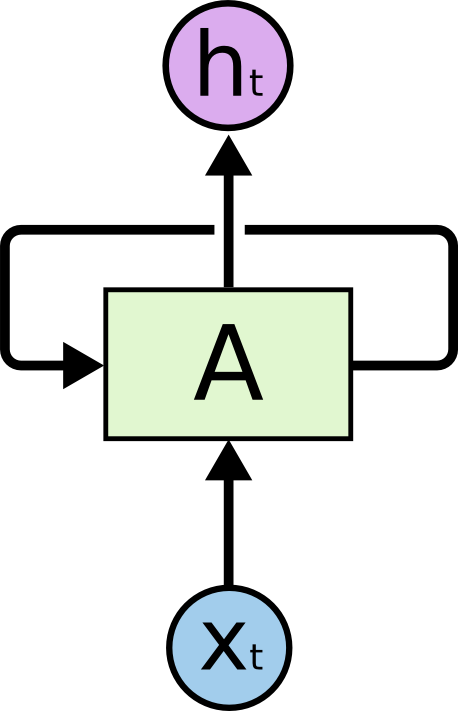
\includegraphics[width = 0.2\textwidth]{images/RNN-rolled.png}
        \caption{RNN-rolled}
        \label{fig:RNN}
    \end{figure}
    
        \begin{lstlisting}
    model = Sequential()

    model.add(LSTM(16, input_shape=(X.shape[1:]), activation='relu', return_sequences=True))
    model.add(Dropout(0.2))
    
    model.add(LSTM(16, activation='relu'))
    model.add(Dropout(0.2))
    
    model.add(Dense(10, activation='relu'))
    model.add(Dropout(0.2))
    
    model.add(Dense(4, activation='softmax'))
    
    opt = tf.keras.optimizers.Adam(lr=0.001, decay=1e-6)
    
    # Compile model
    model.compile(
        loss='sparse_categorical_crossentropy',
        optimizer=opt,
        metrics=['accuracy'],
    )
    \end{lstlisting}
    
    In this article, I will create a 4 layers neural network. First 2 layers is LSTM with 16 cells each and activation layer is rectifier linear unit. The next layer is a dense layer with 10 units. Finally, the output layer has 4 units corresponding to 4 output class that we have discussed before. The figure~\ref{fig:LSTMDiagram} will visualize the structure of this network. We will feed this network with both the dataset with W1 and W2 data to have a nice comparison and see which is the most accurate when apply LSTM.
    

    \begin{figure}[h]
        \centering
        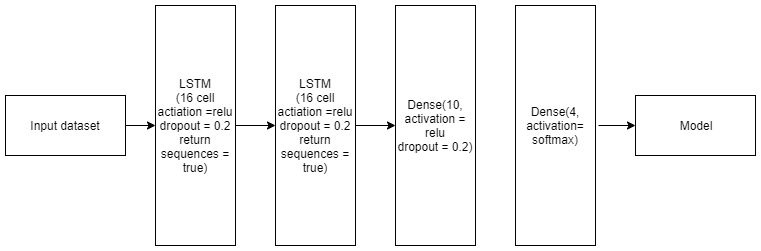
\includegraphics[width = 1\textwidth]{images/LSTMDiagram.png}
        \caption{Neural network breakdown diagram}
        \label{fig:LSTMDiagram}
    \end{figure}
    
    
    \subsection{SVM}
    
     SVM is a very popular supervised machine learning models that from the input data users give do classification and regression. With input data already labeled, the output of SVM is an optimal hyper plane which categorizes new data points~\cite{GG}. For example, in 2D space, hyper plane is a line create the boundary between 2 groups of data. SVM also can work well in multidimensional. 
    
    Scikit learn have already built-in the SVM function and we can easily implement this function. I will use SVC with gamma value is scale for better result. We also will separate 20\% of the dataset we have to create a validate set to check of accuracy of the model. I will leave the default kernel of SVC is radial basis function~\cite{GGG}.